\section{Snap!}
Cette partie donne un aperçu de l'application qui est utilisée dans ce travail. La présentation de \gls{snap} \cite{snap} se diviser en plusieurs paragraphes. La première explique les différents types de \glspl{bloc} et comment ils sont implémentés. L'étape suivante est l'explication de l'exécution d'un programme. Ensuite vient l'affichage les différents éléments de \gls{snap}.

\subsection{Utilisation}
%Cette partie présente comment utiliser \gls{snap} pour faire un programme. Elle présentera le différente division de l'interface graphique ainsi que leur utilité. Pour ce faire les image \ref{fig:snap interface} et \ref{fig:prog} sont utilisé, la première présente les différentes divisions de l'interface, la seconde montre un exemple concret de programme.
Cette partie va illustrer comment réaliser un programme avec \gls{snap} ceci permet de découvrir les différentes zones de l'interface de \gls{snap} et leurs utilisations. Cette explication se base sur les images \ref{fig:snap interface} et \ref{fig:prog}.\\

Pour réaliser un programme avec \gls{snap}, il faut commencer par savoir combien de personnages sont souhaités. Les personnages s'appellent des \textit{\glspl{sprite}} et sont visible dans la \textit{zone des \glspl{sprite}} de la figure \ref{fig:snap interface}. On peut voir dans le programme de l'image \ref{fig:prog}, que deux personnages y sont présent, un chien et un chat. Le bouton blanc au dessus de la \textit{zone de \glspl{sprite}} permet d'ajouter des personnages.\\

Après avoir ajouté le nombre de personnages souhaité, il faut maintenant faire des \glstpl{script} qui seront le code du programme. Les \glstpl{script} sont assemblé, par glissé-déposé, dans la \textit{zone d'édition} au centre de l'interface. Ceux-ci sont construit à l'aide de \gls{bloc} qui se trouve dans la \textit{zone des \glspl{bloc} sources}. Cette zone contient tous les \glspl{bloc} disponibles classés par catégorie suivant l'action du \gls{bloc}.\\

Une fois le programme fini, le drapeau vert dans la \textit{barre d'outils}, lance le programme. Quand le programme est lancé, les actions des \glstpl{script} sont visibles dans la \textit{scène}. Cette zone représente le monde dans lequel va évoluer les personnages. On peut y mettre un fond comme arrière plan ou simplement le laisser blanc comme dans l'exemple, ceci se fait via le bouton stage de la \textit{zone de \glspl{sprite}}.
\paragraph{Barre d'outils}

\begin{figure}
  \begin{center}
  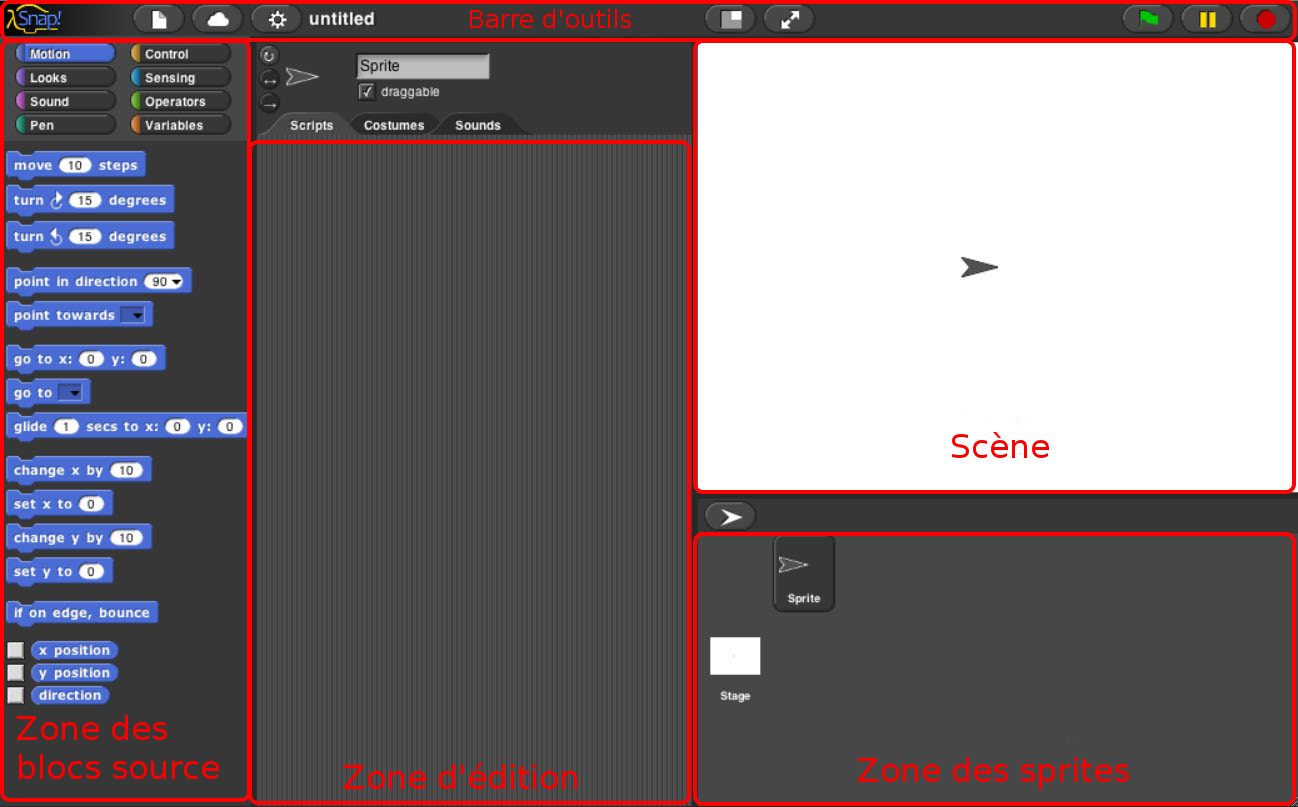
\includegraphics[width=\textwidth]{content/7-solution/2-snap/images/interface}
        \caption{Délimitation des zones de l'interface Snap!}
    \label{fig:snap interface}
  \end{center}
\end{figure}

\subsection{Blocs}
Il existe plusieurs types de \glspl{bloc} qui constituent un programme \gls{snap} \cite{snap-man}. Sur la figure \ref{fig:software-used-script}, le programme présente les différents types \glspl{bloc} disponibles.
\begin{figure}
  \begin{center}
    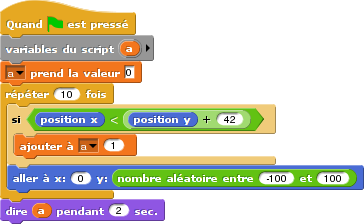
\includegraphics[width=0.5\textwidth]{content/5-related_work/images/script}
    \caption{Exemple de programme Snap!}
    \label{fig:software-used-script}
  \end{center}
\end{figure}

\subsubsection{Commande}
Le type principal de \glspl{bloc} est \texttt{commande}. Ces \glspl{bloc} peuvent être compris comme étant des procédures. En effet, ils exécutent une ou plusieurs opérations sur le système en fonction de paramètres fournis. Ces différents \glspl{bloc} doivent se baser soit sur une implémentation JavaScript pour les \texttt{commande} élémentaires, soit être une composition de \texttt{commande} pour fournir une nouvelle \texttt{commande} plus complexe ou abstraite.

Dans l'exemple de la figure \ref{fig:software-used-script}, tous les \glspl{bloc} \texttt{commande} ont la forme d'une pièce de puzzle. On peut y voir qu'une succession de \texttt{commande} crée un \gls{script}. Les \texttt{commande} ont plusieurs couleurs suivant la catégorie à laquelle elles appartiennent : mouvement, apparence, contrôle, variable \ldots

\subsubsection{Reporter}
Les \texttt{reporter's} sont des fonctions. En effet, ils renvoient une valeur. Ils sont toujours utilisés en temps que paramètres d'un autre \gls{bloc}. La plupart des \texttt{reporter} sont des accesseurs à des variables ou à des états du système (position souris, heure \ldots).

Les \texttt{reporter} sont des \glspl{bloc} de forme arrondie. La figure \ref{fig:software-used-script} montre différentes utilisations de \texttt{reporter} : somme, valeur aléatoire, position, etc. Tout comme pour les \texttt{commande}, les \texttt{reporter} peuvent être de diverses couleurs suivant leur catégorie.

\subsubsection{Prédicat}
Les \texttt{prédicat} sont des reporters qui retournent une valeur booléenne. Ils sont donc utilisés en conjonction avec des commandes demandant une condition. Les \texttt{prédicat} ont une forme hexagonale.
%TODO ajouter un exemple

\subsubsection{Chapeau}
Les \texttt{chapeau} sont des commandes spéciales car ils sont le point d'entrée obligatoire d'un \gls{script} en permettant de démarrer l'exécution de celui-ci. Plusieurs types d'événements peuvent lancer un \gls{script} : une touche pressée, un clic sur le drapeau vert.

Dans la figure \ref{fig:software-used-script}, le démarrage du programme est l'événement qui lance le \gls{script}. Il est symbolisé par un drapeau vert.

\subsection{Programme}
\gls{snap} est plus qu'une interface graphique permettant de construire un programme. L'analyse de son fonctionnement interne est l'objet de ce paragraphe.

Un programme est constitué de plusieurs processus. Chaque processus est exécuté en parallèle grâce à un ordonnanceur.

% /*
%     A Process is what brings a stack of blocks to life. The process
%     keeps track of which block to run next, evaluates block arguments,
%     handles control structures, and so forth.
%
%     The ThreadManager is the (passive) scheduler, telling each process
%     when to run by calling its runStep() method. The runStep() method
%     will execute some number of blocks, then voluntarily yield control
%     so that the ThreadManager can run another process.
%
%     The Scratch etiquette is that a process should yield control at the
%     end of every loop iteration, and while it is running a timed command
%     (e.g. "wait 5 secs") or a synchronous command (e.g. "broadcast xxx
%     and wait"). Since Snap also has lambda and custom blocks Snap adds
%     yields at the beginning of each non-atomic custom command block
%     execution, and - to let users escape infinite loops and recursion -
%     whenever the process runs into a timeout.
%
%     a Process runs for a receiver, i.e. a sprite or the stage or any
%     blocks-scriptable object that we'll introduce.
%
%     structure:
%
%     topBlock            the stack's first block, of which all others
%                         are children
%     receiver            object (sprite) to which the process applies,
%                         cached from the top block
%     context                the Context describing the current state
%                         of this process
%     homeContext            stores information relevant to the whole process,
%                         i.e. its receiver, result etc.
%     isPaused            boolean indicating whether to pause
%     readyToYield        boolean indicating whether to yield control to
%                         another process
%     readyToTerminate    boolean indicating whether the stop method has
%                         been called
%     isDead              boolean indicating a terminated clone process
%     timeout                msecs after which to force yield
%     lastYield            msecs when the process last yielded
%     errorFlag            boolean indicating whether an error was encountered
%     prompter            active instance of StagePrompterMorph
%     httpRequest         active instance of an HttpRequest or null
%     pauseOffset         msecs between the start of an interpolated operation
%                         and when the process was paused
% */

Un processus \texttt{Process} représente l'exécution d'un \gls{script}, une pile de \glspl{bloc}. Il assure aussi le suivi de l'exécution du \gls{script} : prochain \gls{bloc} à exécuter, objet sur lequel il s'applique, contexte décrivant l'état courant, etc.

L'ordonnanceur \texttt{ThreadManager} appelle la fonction \texttt{runStep()} (extrait de code source \ref{lst-runstep}) successivement sur chaque processus. Cette fonction exécute un certain nombre de \glspl{bloc} via \texttt{this.evaluateContext()} de manière atomique. Elle rend la main volontairement à l'ordonnanceur quand elle a fini. Comme il est possible d'écrire soi-même des \glspl{bloc}, \texttt{runStep()} rend aussi la main si trop de temps s'est écoulé depuis le début de l'exécution de cette étape. La convention veut que les processus rendent la main à la fin de chaque itération de boucles et quand une opération relative au temps ou synchrone est exécutée.
\begin{figure}
\begin{lstlisting}[caption={Fonction \texttt{runStep()} de \texttt{Process}},label=lst-runstep,language=JavaScript]
Process.prototype.runStep = function () {
/*
    a step is an an uninterruptable 'atom', it can consist
    of several contexts, even of several blocks
*/
    // allow pausing in between atomic steps:
    if (this.isPaused) {
        return this.pauseStep();
    }
    this.readyToYield = false;
    while (!this.readyToYield
            && this.context
            && (this.isAtomic ? (Date.now() - this.lastYield < this.timeout) : true) ) {
        // also allow pausing inside atomic steps - for PAUSE block primitive:
        if (this.isPaused) {
            return this.pauseStep();
        }
        this.evaluateContext();
    }
    this.lastYield = Date.now();

    // make sure to redraw atomic things
    if (this.isAtomic &&
            this.homeContext.receiver &&
            this.homeContext.receiver.endWarp) {
        this.homeContext.receiver.endWarp();
        this.homeContext.receiver.startWarp();
    }

    if (this.readyToTerminate) {
        while (this.context) {
            this.popContext();
        }
        // pen optimization
        if (this.homeContext.receiver &&
                this.homeContext.receiver.endWarp) {
            this.homeContext.receiver.endWarp();
        }
    }
};
\end{lstlisting}
\end{figure}


% /*
%     A Context describes the state of a Process.
%
%     Each Process has a pointer to a Context containing its
%     state. Whenever the Process yields control, its Context
%     tells it exactly where it left off.
%
%     structure:
%
%     parentContext    the Context to return to when this one has
%                     been evaluated.
%     outerContext    the Context holding my lexical scope
%     expression        SyntaxElementMorph, an array of blocks to evaluate,
%                     null or a String denoting a selector, e.g. 'doYield'
%     receiver        the object to which the expression applies, if any
%     variables        the current VariableFrame, if any
%     upvars          the current UpvarReference, if any (default: null)
%     inputs            an array of input values computed so far
%                     (if expression is a    BlockMorph)
%     pc                the index of the next block to evaluate
%                     (if expression is an array)
%     startTime        time when the context was first evaluated
%     startValue        initial value for interpolated operations
%     activeAudio     audio buffer for interpolated operations, don't persist
%     activeNote      audio oscillator for interpolated ops, don't persist
%     isLambda        marker for return ops
%     isImplicitLambda    marker for return ops
%     isCustomBlock   marker for return ops
%     emptySlots        caches the number of empty slots for reification
% */

\subsection{Interface graphique}
Un autre élément intéressant à analyser chez \gls{snap} est sa façon d'afficher l'interface dans la balise HTML \texttt{canvas} (voir code source \ref{lst-doonecycle}). Toutes les fonctionnalités de bases nécessaires à afficher tous les éléments graphiques de \gls{snap} découlent de l'implémentation que l'on retrouve dans \texttt{morphic.js}.

\texttt{morphic.js} fournit les abstractions pour redessiner des parties de l'interface et pour interagir avec l'utilisateur. Le \texttt{canvas} utilisé possède un \texttt{world}. Ce \texttt{world} est la racine de l'arbre composé de \texttt{morph} et leurs sous-\texttt{morph}. Chaque \texttt{morph} peut être déplacé, redimensionné via le code source ou les manipulations de l'utilisateur.

La fonction principale de \texttt{morphic.js} consiste à parcourir continuellement tous les éléments du \texttt{world} pour redessiner ceux qui ont été modifiés. Le \texttt{world} permet à l'ordonnanceur d'exécuter une étape entre chaque itération. Le code source \ref{lst-doonecycle} montre que le monde est rafraîchit toutes les 50 millisecondes.
\begin{figure}
\begin{lstlisting}[caption={Exemple d'utilisation de \texttt{morphic.js}},label=lst-doonecycle,language=HTML5,alsolanguage=JavaScript]
<!DOCTYPE html>
<html>
    <head>
        <title>Morphic!</title>
        <script type="text/javascript" src="morphic.js"></script>
        <script type="text/javascript">
            var world;

            window.onload = function () {
                world = new WorldMorph(
                    document.getElementById('world'));
                setInterval(loop, 50);
            };

            function loop() {
                world.doOneCycle();
            }
        </script>
    </head>
    <body>
        <canvas id="world" tabindex="1" width="800" height="600" />
    </body>
</html>
\end{lstlisting}
\end{figure}
La fonction \texttt{drawNew()} sert à dessiner un \texttt{morph}. Le code source \ref{lst-drawnew} montre que cette fonction dessine son objet sur une image stockée dans l'objet. Cette image provient d'un \texttt{canvas} virtuel généré grâce à l'image du \texttt{morph} parent.

\begin{figure}
\begin{lstlisting}[caption={Modèle pour la fonction \texttt{drawNew()}},label=lst-drawnew,language=JavaScript]
MyMorph.prototype.drawNew = function() {
    var context;
    this.image = newCanvas(this.extent());
    context = this.image.getContext('2d');
    // use context to paint stuff here
};
\end{lstlisting}
\end{figure}

\section{Ruby on Rails}
\label{rails}
\gls{rails} \cite{rails} est une plateforme de développement d'application web basée sur le langage de programmation Ruby \cite{ruby}. Cette partie présente la philosophie, l'architecture et des environnements de tests de \gls{rails}.

\subsection{Philosophie}
\gls{rails} part de l'hypothèse qu'il existe une meilleure façon d'aborder la création d'application web \cite{rails-guides}. Si le programmeur respecte ce "Rails way", il améliorera sa productivité et écrira moins de code. D'après \gls{rails}, s’il persiste à utiliser ses anciennes habitudes, le développeur s'amusera beaucoup moins en créant son application.

Pour atteindre cet objectif, Rails utilise deux principes majeurs :
\begin{description}
  \item[Convention plutôt que configuration (CoC) \cite{wiki-coc}] Pour permettre au programmeur d'écrire moins de code, \gls{rails} permet de n'écrire que ce qui ne correspond pas aux conventions. \gls{rails} utilise la métaprogrammation pour fournir les conventions à tous les objets ;
  \item[Ne vous répétez  pas (DRY) \cite{wiki-dry}] \gls{rails} recommande une architecture où il faut mettre l'information à un endroit unique et bien déterminé. Ceci permet d'avoir un code plus court, plus maintenable, plus extensible et avec moins de bogues.
\end{description}

\label{rbp}
Un service aidant à mieux comprendre et respecter le "Rails way" présenté plus tôt est Rails\_best\_practices. Il fournit des métriques utiles pour détecter des écarts à la philosophie \gls{rails}. Cet outil s'utilise avec les conseils fournis par \url{http://rails-bestpractices.com} aidant à refactorer les morceaux de code qui ne respecteraient pas les conventions.

\subsection{Architecture}
\gls{rails} se base sur une architecture \gls{mvc} \cite{wiki-mvc} (figure \ref{fig:mvc}).
\begin{figure}[ht]
  \begin{center}
    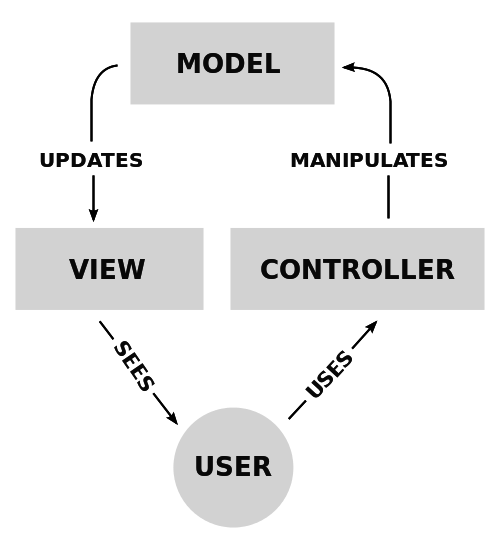
\includegraphics[scale=0.3]{content/4-prerequis/images/mvc}
    \caption{Schéma interaction d'un modèle MVC}
    \label{fig:mvc}
  \end{center}
\end{figure}
\subsubsection{Modèle}
Un modèle est typiquement une classe qui représente une table de la base de données. Une classe du modèle fournit aussi toutes les méthodes nécessaires à représenter et modifier l'objet dans le domaine d'application.

La correspondance entre un objet Ruby et la base de données est réalisée grâce à \textit{Active Record}. Ce module de \gls{rails} permet de faire des appels sur des objets Ruby alors que dans d'autres framework, il faudrait utiliser des requêtes \textit{SQL}. \label{active-record}

\subsubsection{Contrôleur}
\label{controleur}
Le contrôleur a pour fonction d'accéder à une ressource. Une ressource est un modèle ou tout autre objet indirect tel que enregistrement, login, page d'accueil\ldots

Il détermine quelle vue doit s'afficher et avec quels paramètres. Le contrôleur a donc la tâche de vérifier la sécurité et l'intégrité des données fournies par l'utilisateur. Ensuite, il peut interroger différents modèles et fournir les réponses à la vue adéquate.

\label{rest}\label{rails-routes}
\gls{rails} encourage d'avoir des ressources \gls{rest} \cite{wiki-rest}, c'est-à-dire, des ressources avec une représentation unique et des actions unifiées telles que create, new, edit, update, destroy, show, index. Les actions disponibles sur un contrôleur sont déterminées par le fichier de configuration des routes.

\subsubsection{Vue}
Les vues correspondent à ce que les utilisateurs reçoivent et voient. Ce sont typiquement des pages HTML, mais aussi des PDF, objets JSON, fichiers, etc\ldots

Pour faciliter la création des vues, \gls{rails} permet d'utiliser des \glspl{gem}. Il existe notamment:
\begin{description}
  \item[Haml \cite{haml} \label{haml}] un langage fournissant une syntaxe raccourcie du HTML. Il se base sur l'indentation plutôt que sur une syntaxe XML. Haml permet donc de respecter le principe \texttt{DRY} et d'améliorer la lisibilité par un code source plus court et bien indenté ;
  \item[JQuery \cite{jquery}] cette bibliothèque javaScript bien connue permet de modifier facilement le document courant, de gérer des événements, de créer des animations, etc. ;
  \item[CoffeeScript \cite{coffeescript}] est un langage qui se compile en JavaScript. Il permet d'avoir une syntaxe plus claire, plus courte et d'ajouter des sucres syntaxiques par rapport à JavaScript;
  \item[Bootstrap \cite{bootstrap}] est un framework CSS qui découple le fond et la forme de l'affichage d'une page HTML. Ce framework donne un design adaptatif pour tous types d'écrans aux pages qui l'utilisent. Il fournit aussi de nombreux composants utiles : boutons, alertes, barres de progression, messages d'aide, etc. \label{bootstrap}
\end{description}
%TODO intégré avec les contrôleurs. Paperclip dans les vues
\subsection{Gems}
\label{gems}
Ruby fournit une manière de partager des fonctionnalités pour des programmes Ruby via les \glspl{gem} \cite{gem}. \gls{rails} lui-même est un \gls{gem} et dépend de nombreux autres notamment Active Record présentés plus haut.

\label{gemnasium}
La communauté de \gls{rails} a écrit de nombreux \glspl{gem}  permettant de rajouter facilement des fonctionnalités à une application. Le fichier \texttt{Gemfile} sert à lister les \glspl{gem}  utilisé dans un projet. Le gestionnaire du projet, doit faire attention à toutes ces dépendances pour garder son logiciel à jour. Pour ce faire, Gemnasium analyse le fichier \texttt{Gemfile} pour indiquer quel \glspl{gem}  doivent être mis à jours. Gemnasium informe donc les gestionnaires d'un logiciel lorsqu'une faille de sécurité est découverte dans un \gls{gem} et qu'il faut donc le mettre à jour.

Quelque exemples de \glspl{gem} intéressants sont présentées ci-après.
\begin{description}
  \item[Paperclip \cite{paperclip}] permet de facilement récupérer et stocker des fichiers. Paperclip intègre donc la gestion de fichiers tiers de manière élégante dans une classe du modèle. Il fournit notamment divers pilotes pour stocker ces fichiers aussi bien en local que sur le nuage d'amazon ou de dropbox.
  \item[Devise \cite{devise}] gère la problématique de l'authentification des utilisateurs.
  \item[Rolify \cite{rolify}] donne des \glspl{role} aux utilisateurs de manière générale (ex. administrateur) ou sur une ressource (ex. modérateur d'un forum).\label{rolify}
  \item[Authority \cite{authority}] gère les droits des utilisateurs sur les différentes ressources des contrôleurs. \label{authority}
\end{description}

\subsection{Tests}
\label{rails-tests}
Il existe tout un écosystème autour de \gls{rails} pour fournir du code de qualité. Cette partie présente quelques outils utilisés dans les tests. Les outils les plus employés seront présentés ci-dessous, bien que ce ne soit pas les seuls existants.

\subsubsection{Tests comportementaux}
\label{cucumber}
Un outil de test fort apprécié des programmeurs Ruby et plus particulièrement \gls{rails} est Cucumber \cite{cucumber}. Ce dernier réalise des tests dans un "behavior-driven development" \cite{wiki-bdd} style. Ce style de tests se compose de deux parties. D'une part, le client ou chef de projet écrit des scénarii qui décrivent l'utilisation de fonctionnalités du domaine en langage naturel (Gherkin \cite{gherkin}). D'autre part, le programmeur implémente ces scénarii. Ce type de test met l'accent sur ce que voit le client. Si tout ce que voit le client fonctionne, c'est que le coeur utile de l'application est correct.

Dans le cas de \gls{rails}, il est intéressant d'utiliser conjointement Cucumber et Capybara \cite{capybara}. Ce dernier permet de contrôler un navigateur et donc de réaliser des tests à la place d'un utilisateur. Ces tests permettront d'assurer le bon fonctionnement de ce que souhaite l'utilisateur.

\subsubsection{Intégration continue}
\label{travis}
Dans le cadre d'un développement actif, il est intéressant d'avoir un serveur qui réalise des tests d'intégration continue \cite{wiki-int-cont}. En effectuant les tests lors de chaque nouveau \texttt{commit}, les développeurs sont informés directement si une modification du code source a induit une régression des fonctionnalités. Ce service est proposé entre autres par \texttt{Travis CI}\cite{travis}.
